%Correct the file name.
%X: book number
%Y: part number
%ZZZ: page number in three digits. So page 3 would be 003.

\documentclass[11pt]{amsbook}

\usepackage{../HBSuerDemir}	% ------------------------
\usepackage{booktabs}

\begin{document}

% ++++++++++++++++++++++++++++++++++++++
\hPage{b2p1/049}
% ++++++++++++++++++++++++++++++++++++++

\begin{center}
	\begin{tabular}{l}
	\begin{tabular}{c c c c c c}
		$n  : $ & $0$ & $1$ & $2$ & $3$ & $4$ \\
		\midrule
		$a_n :$ & $0$ & $1$ & $-\frac{1}{2}$ & $\frac{1}{3}$ & $-\frac{1}{4}$
		\\
		$b_n : $ & $0$ & $1$ & $0$ & $-\frac{1}{6}$ & $0$ \\
		\midrule
		$p_n : $ & $0$ & $0$ & $1$ & $-\frac{1}{2}$ & $\frac{1}{6}$
	\end{tabular}
	\\
	$[\ln(1+x)]\sin x = x^2 - \frac{1}{2}x^3 + \frac{1}{6}x^4 + \ldots$
\end{tabular}
\end{center}

\noindent
where the general term is omitted since it is unnecessary, and we have all properties of the series, because, those of $\ln(x+1)$ and $\sin x$ are known.

Example 4. Obtain power series expansions of the following rational functions at the indicated points:
		
	a ) $\frac{3+x}{1-x} , x = 0$ 
	b ) $\frac{3+x}{x} , x = 1$
	
Solution.
	\newline
	a ) Direct division gives (since $b_0 = 1 \neq 0$)

	\begin{center}
		$\frac{3+x}{1-x} = 3 + 4x + 4x^2 + \ldots + 4x^n + \ldots$ .
	\end{center}

\noindent
Observe that it involves a geometric series with common ratio x. Then it is convergent for $|x|<1$.
\newline
	Obtain the same series by performing
	\begin{center}
		$(3 + x)(1 + x + \ldots + x^n + \ldots)$,
	\end{center}
\noindent
and also by differentiating $(3+x)(1-x)$ successively at $x = 0$.

b ) The series being in powers of  $x - 1$, use substitution $x - 1 = t$ or $x = 1 + t$. Then
\begin{center}
	$\frac{3+x}{x} = \frac{3+(1+t)}{1+t} = \frac{4+t}{1+t} = 4 - 3t + 3t^2 - \ldots + (-1)^n 3t^n - \ldots$
	\newline
	$= 4 - 3(x-1) + 3(x-1)^2 - \ldots + (-1)^n 3(x-1)^n - \ldots$
\end{center}
\noindent
convergent for $|x-1|<1$.

% =======================================================
\end{document}  

%==== templates ====

%==== environments ====

%\begin{figure}[htb]
%	\centering
%	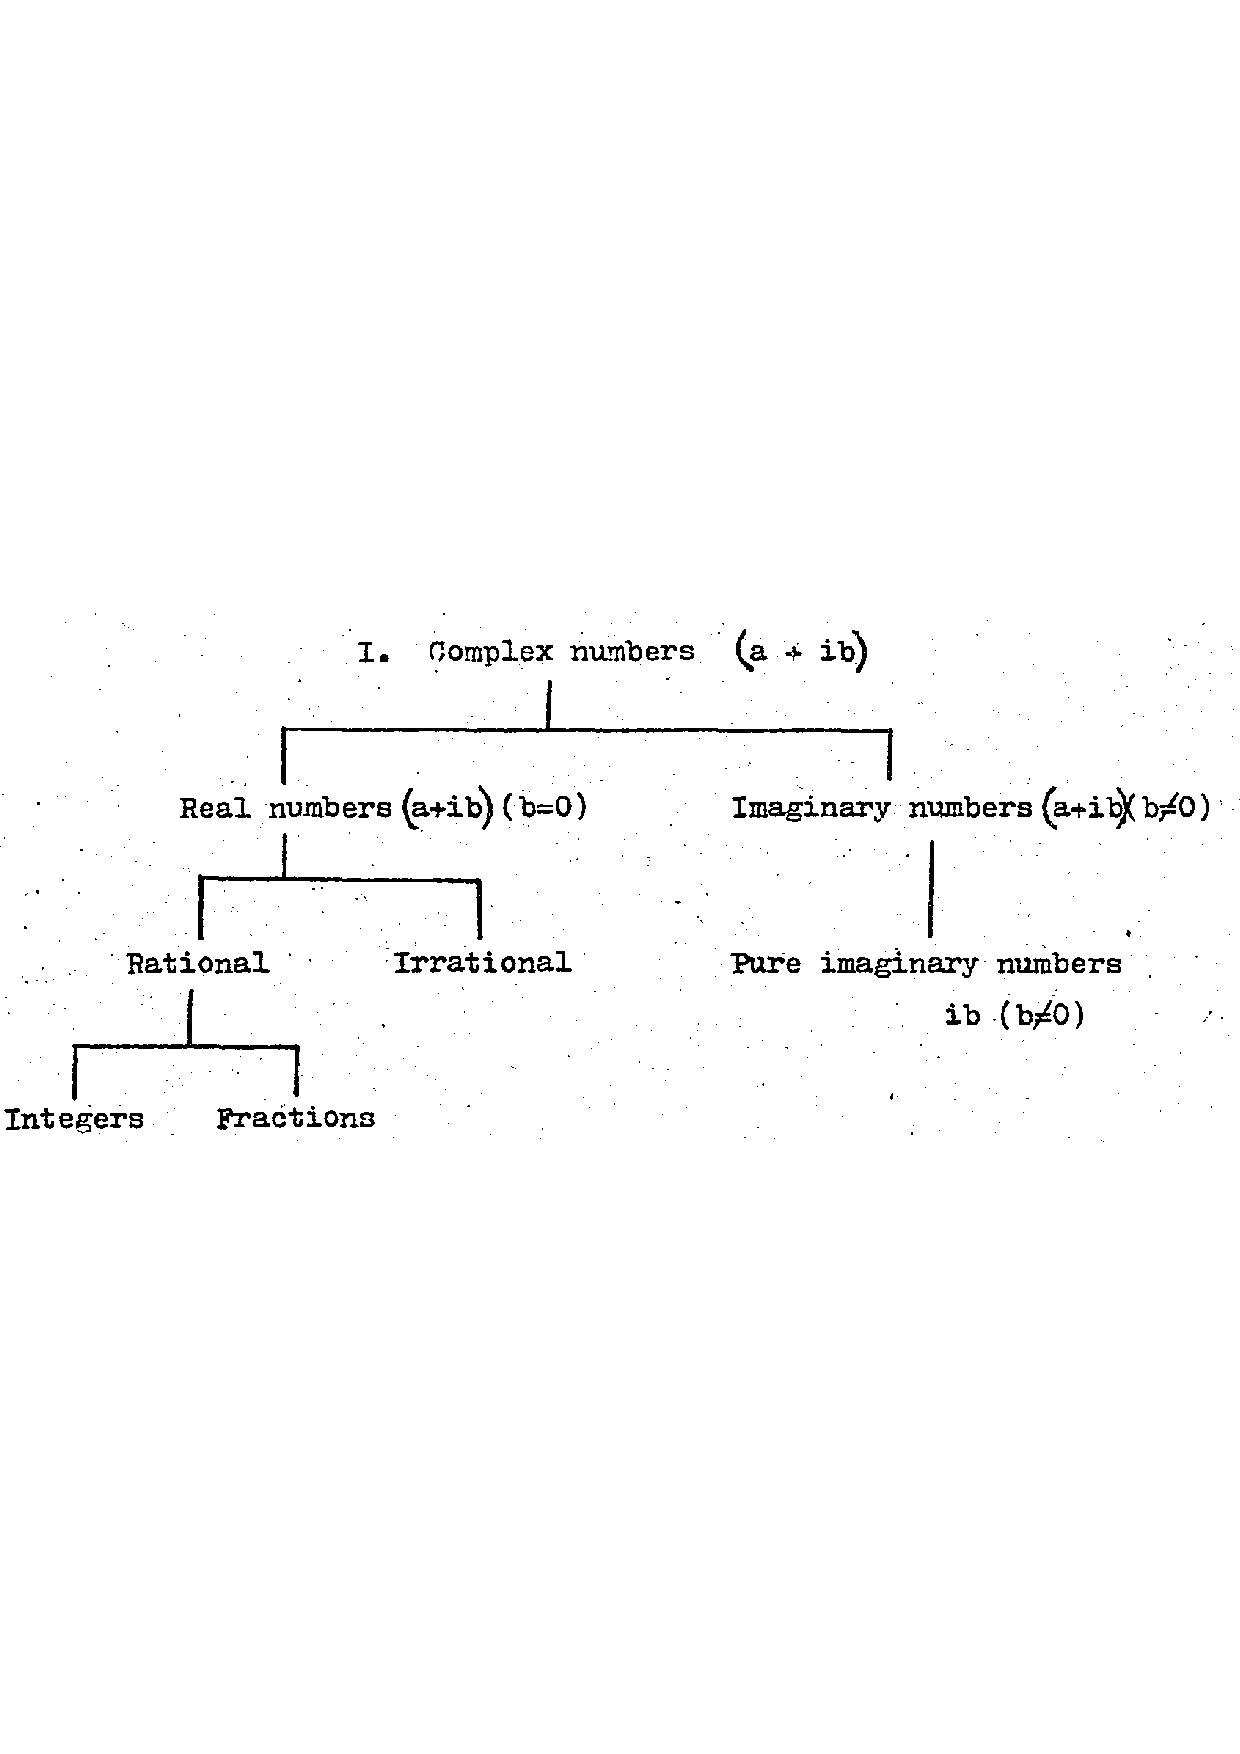
\includegraphics[width=0.9\textwidth]{images/SD-1-1p15A}
%	\caption{Classification of complex numbers}
%	\label{fig:classificationOfComplexNumbersA}
%\end{figure}

%\begin{center}
%\begin{tabular}{cc}
%\end{tabular}
%\end{center}

%\begin{exmp}
%\begin{hSolution}
%\end{hSolution}
%\end{exmp}

%\begin{hEnumerateAlpha}
%\end{hEnumerateAlpha}

%\begin{hEnumerateRoman}
%\end{hEnumerateRoman}

%$
%\begin{bmatrix}
%\end{bmatrix}
%$

%\frac{aaaa}{bbb}
%\frac{a_{n}}{b_{n}}
%\left( aaaa \right)
%\Longrightarrow

%\begin{multicols}{2}
%	bb
%\columnbreak
%	aa
%\end{multicols}
